\begin{frame}
	\myheading{Module 13.10 : Fooling Deep Convolution Neural Networks}
\end{frame}

%%%%%%%%%%%%%%%%%%%%%%%%%%%%%%%%%%%%%%%%%%%%%%%%%%%%%%%%%%%%%%%%%%%%%%%%%%%%%%%%%%%%%%%%%

\begin{frame}	
	\vspace{1cm}
	
	\begin{overlayarea}{\textwidth}{\textheight}
		\begin{block}{}
			\begin{itemize}
				\justifying
				\onslide<1->{
					\item Turns out that using this idea of optimizing over the input, we can also ``fool" ConvNets
					}	
					\onslide<2->{ 
						\item Let us see how
					}			
			\end{itemize}
		\end{block}		
	\end{overlayarea}		
	
\end{frame}

%%%%%%%%%%%%%%%%%%%%%%%%%%%%%%%%%%%%%%%%%%%%%%%%%%%%%%%%%%%%%%%%%%%%%%%%%%%%%%%%%%%%%%%%%

\begin{frame}
  \begin{columns}
    \column{0.5\textwidth}
            \hspace{-0.8cm}
    \begin{overlayarea}{\textwidth}{\textheight}
        %\PassOptionsToClass{}{beamer}
\documentclass[serif,aspectratio=169,dvipsnames]{beamer}
\usepackage[utf8]{inputenc}

%\StartShownPreambleCommands
\usepackage{amsmath,esint}
\usepackage{amssymb}
\usepackage[british]{babel}
\usepackage{multicol}
\usetheme{Warsaw}
\usecolortheme{rose}
\usepackage[normalem]{ulem}
%\usetheme{metropolis}
%\usepackage{appendixnumberbeamer}

%\StopShownPreambleCommands
\usepackage{pgfplots}

\usepackage{ mathrsfs }
\usepackage{hyperref}

\usepackage{gensymb}
\usepackage{color}
\usepackage{tkz-euclide}
\usetkzobj{all}
\usepackage{tkz-fct}  
\usetikzlibrary{calc}
\usepackage{ragged2e}
\usepackage[ruled]{algorithm2e}
\usepackage{tikz}
\usepackage{animate}
\usepackage{adjustbox}
\usepackage[labelformat=empty]{caption}
\usepackage{blindtext}
\usepackage{biblatex}


\usetikzlibrary{matrix,chains,positioning,decorations.pathreplacing,arrows} 
\usetikzlibrary{shapes.geometric}
\usetikzlibrary{intersections}


\makeatletter

\DeclareMathOperator*{\minimize}{minimize}

\newcommand\myheading[1]{%
\par\bigskip
{\Large\bfseries#1}\par\smallskip}


\addtobeamertemplate{navigation symbols}{}{%
    \usebeamerfont{footline}%
    \usebeamercolor[fg]{footline}%
    \hspace{1em}%
    \insertframenumber/\inserttotalframenumber
}

\setbeamertemplate{title page}
{
  \vspace{0.3in}
  \vbox{}
   %{\usebeamercolor[fg]{titlegraphic}\inserttitlegraphic\hfill\inserttitlegraphicii\par}
  \begin{centering}
    \begin{beamercolorbox}[sep=8pt,center]{title}
      \usebeamerfont{title}\inserttitle\par%
      \ifx\insertsubtitle\@empty%
      \else%
        \vskip0.25em%
        {\usebeamerfont{subtitle}\usebeamercolor[fg]{subtitle}\insertsubtitle\par}%
      \fi%     
    \end{beamercolorbox}%
    \vskip1em\par
    \begin{beamercolorbox}[sep=8pt,center]{date}
      \usebeamerfont{date}\insertdate
    \end{beamercolorbox}%\vskip0.5em
    \begin{beamercolorbox}[sep=8pt,center]{author}
      \usebeamerfont{author}\insertauthor
    \end{beamercolorbox}
    \begin{beamercolorbox}[sep=8pt,center]{institute}
      \usebeamerfont{institute}\insertinstitute
    \end{beamercolorbox}
  \end{centering}
  %\vfill
}
\makeatother

\author{Mitesh M. Khapra}
\title{CS7015 (Deep Learning) : Lecture 18}
\subtitle{Markov Networks}
\institute{Department of Computer Science and Engineering\\ Indian Institute of Technology Madras}
\date{}
\titlegraphic{\includegraphics[height=1cm,width=2cm]{images/iitm_logo.png}}

\begin{document}


\tikzstyle{input_neuron}=[circle,draw=red!50,fill=orange!10,thick,minimum size=1mm]
\tikzstyle{hidden_neuron}=[circle,draw=blue!50,fill=blue!10,thick,minimum size=10mm]
\tikzstyle{output_neuron}=[circle,draw=green!50,fill=green!20,thick,minimum size=4mm]

\tikzstyle{input}=[circle,draw=black!50,fill=black!20,thick,minimum size=.2mm]
\tikzstyle{neuron}=[circle,draw=blue!50,fill=blue!20,thick,minimum size=10mm]
\tikzstyle{neuron1}=[circle,draw=blue!50,fill=cyan!10, thick,minimum size=10mm]
\begin{frame}
	\myheading{Module 18.3: Local Independencies in a Markov Network}
\end{frame}

\begin{frame}
	\begin{columns}
		\column{0.5\textwidth}
		\begin{overlayarea}{\textwidth}{\textheight}
		\end{overlayarea}
		\column{0.5\textwidth}
		\begin{overlayarea}{\textwidth}{\textheight}
			\begin{itemize}[<+->]\justifying
				\item Let $U$ be the set of all random variables in our joint distribution 
				\item Let $X,Y,Z$ be some distinct subsets of $U$
				\item A distribution $P$ over these RVs would imply $X\bot Y|Z$ if and only if we can write 
				\begin{align*}
				P(X) = \phi_1(X,Z)\phi_2(Y,Z)
				\end{align*}
				\item Let us see this in the context of our original example
			\end{itemize}
		\end{overlayarea}
	\end{columns}
\end{frame}

\begin{frame}
	\begin{columns}
		\column{0.5\textwidth}
		\begin{overlayarea}{\textwidth}{\textheight}
			\begin{center}
					\tikzstyle{input_neuron}=[circle,draw=red!50,fill=orange!10,thick]
					\begin{tikzpicture}
						\node [input_neuron](input0) at (5.5,-0.1)  {D};
						\node [input_neuron] (input1) at (9.5,-0.1)  {B};
						\node [input_neuron] (input2) at (7.5, 1.1) {A};
						\node [input_neuron] (input3) at (7.5, -1.1) {C};
						
						\draw [line width=0.2mm, -] (input0) -- (input2);
						\draw [line width=0.2mm, -] (input0) -- (input3);
						\draw [line width=0.2mm, -] (input1) -- (input2);
						\draw [line width=0.2mm, -] (input1) -- (input3);
					\end{tikzpicture}
				\end{center}

		\end{overlayarea}
		\column{0.5\textwidth}
		\begin{overlayarea}{\textwidth}{\textheight}
			\begin{itemize}[<+->]\justifying
				\item In this example
				\begin{align*}
					&P(A,B,C,D) =\\
					&\frac{1}{Z} [ \phi_1(A,B) \phi_2(B,C) \phi_3(C,D) \phi_4(D,A)]
				\end{align*}
				\item We can rewrite this as 
				\begin{align*}
					&P(A,B,C,D) =\\
					&\frac{1}{Z} \underbrace{[ \phi_1(A,B) \phi_2(B,C) ]}_{\phi_5(B,\{A,C\})} \underbrace{[\phi_3(C,D) \phi_4(D,A)]}_{\phi_6(D,\{A,C\})}
				\end{align*}
				\item We can say that $B \bot D|\{A,C\}$ which is indeed true
			\end{itemize}
		\end{overlayarea}
	\end{columns}
\end{frame}

\begin{frame}
	\begin{columns}
		\column{0.5\textwidth}
		\begin{overlayarea}{\textwidth}{\textheight}
			\begin{center}
					\tikzstyle{input_neuron}=[circle,draw=red!50,fill=orange!10,thick]
					\begin{tikzpicture}
						\node [input_neuron](input0) at (5.5,-0.1)  {D};
						\node [input_neuron] (input1) at (9.5,-0.1)  {B};
						\node [input_neuron] (input2) at (7.5, 1.1) {A};
						\node [input_neuron] (input3) at (7.5, -1.1) {C};
						
						\draw [line width=0.2mm, -] (input0) -- (input2);
						\draw [line width=0.2mm, -] (input0) -- (input3);
						\draw [line width=0.2mm, -] (input1) -- (input2);
						\draw [line width=0.2mm, -] (input1) -- (input3);
					\end{tikzpicture}
				\end{center}
		\end{overlayarea}
		\column{0.5\textwidth}
		\begin{overlayarea}{\textwidth}{\textheight}
			\begin{itemize}[<+->]\justifying
				\item In this example
				\begin{align*}
					&P(A,B,C,D) = \\
					&\frac{1}{Z} [ \phi_1(A,B) \phi_2(B,C) \phi_3(C,D) \phi_4(D,A)]
				\end{align*}
				\item Alternatively we can rewrite this as 
				\begin{align*}
					&P(A,B,C,D) = \\
					&\frac{1}{Z} \underbrace{[ \phi_1(A,B) \phi_2(D,A) ]}_{\phi_5(A,\{B,D\})} \underbrace{[\phi_3(C,D) \phi_4(B,C)]}_{\phi_6(C,\{B,D\})}
				\end{align*}
				\item We can say that $A \bot C|\{B,D\}$ which is indeed true
			\end{itemize}
		\end{overlayarea}
	\end{columns}
\end{frame}

\begin{frame}
	\begin{columns}
		\column{0.5\textwidth}
		\begin{overlayarea}{\textwidth}{\textheight}
			\centering
			\vspace{1cm}\
			\tikzset{mystyle/.style={shape=circle,fill=black,scale=0.3}}
			\tikzset{neigh/.style={shape=circle,fill=blue,scale=0.5}}
			\tikzset{cent/.style={shape=circle,fill=red,scale=0.5}}
			\tikzstyle{input_neuron}=[circle,draw=red!50,fill=orange!10,thick,minimum size=3mm]
			\begin{tikzpicture}[scale=.8]
            % setup the nodes
            \foreach \x in {0,...,5}
            \foreach \y in {0,...,5}
            {
            \ifnum\x=3
                \ifnum\y=2
                    \node[cent] (\x-\y) at (\x,\y){};
                \else
                    \node[mystyle] (\x-\y) at (\x,\y){};
                \fi
            \else
                \node[mystyle] (\x-\y) at (\x,\y){};
            \fi
            }
            % circle selected nodes with letters
            \foreach \mynode/\mytext in {2-2/A,3-3/B,3-1/C,4-2/D}
            {
                \draw[neigh] (\mynode) circle (0.2cm) node {};
            }
			\draw [line width=0.2mm, -] (2.1,2) -- (2.9,2);
			\draw [line width=0.2mm, -] (3,2.9) -- (3,2.1);
			\draw [line width=0.2mm, -] (3,1.1) -- (3,1.9);
			\draw [line width=0.2mm, -] (3.9,2) -- (3.1,2);
	        \end{tikzpicture}
		\end{overlayarea}
		\column{0.5\textwidth}
		\begin{overlayarea}{\textwidth}{\textheight}
			\begin{itemize}[<+->]\justifying
				\item For a given Markov network $H$ we define Markov Blanket of a RV $X$ to be the neighbors of $X$ in $H$
				\item Analogous to the case of Bayesian Networks we can define the local independences associated with $H$ to be
				\begin{align*}
					\color{red} X \color{black} \bot (U - \{X\} - MB_H) | \color{blue}MB_H(X)\color{black}
				\end{align*}  
			\end{itemize}
		\end{overlayarea}
	\end{columns}
\end{frame}

\begin{frame}
	\begin{columns}
		\column{0.5\textwidth}
		\begin{overlayarea}{\textwidth}{0.7\textheight}
			\begin{center}
			Bayesian network
			\end{center}
			\begin{center}
				\tikzstyle{input_neuron}=[ellipse,draw=red!50,fill=orange!10,thick,scale=0.7]
				\begin{tikzpicture}
					\node [input_neuron](input0) at (7,-0.1)  {Grade};
					\node [input_neuron] (input1) at (10,-0.1)  {SAT};
					\node [input_neuron] (input2) at (8.5, 1.1) {Intellligence};
					\node [input_neuron] (input3) at (7, -1.1) {Letter};
					\node [input_neuron](input4) at (5.5,1.1)  {Difficulty};

					\draw [line width=0.2mm, ->] (input2) -- (input0);
					\draw [line width=0.2mm, ->] (input0) -- (input3);
					\draw [line width=0.2mm, ->] (input2) -- (input1);
					\draw [line width=0.2mm, ->] (input4) -- (input0);
				\end{tikzpicture}
			\end{center}
	        \vspace{0.4cm}
			Local Independencies 
			\begin{align*}
				X_i \bot NonDescendents_{X_i} | Parent_{X_i}^G
			\end{align*}

		\end{overlayarea}
		\column{0.5\textwidth}
		\begin{overlayarea}{\textwidth}{0.7\textheight}
			\begin{center}
			Markov network\\
			\vspace{0.2cm}
			\tikzset{mystyle/.style={shape=circle,fill=black,scale=0.3}}
			\tikzset{neigh/.style={shape=circle,fill=blue,scale=0.5}}
			\tikzset{cent/.style={shape=circle,fill=red,scale=0.5}}
			\tikzstyle{input_neuron}=[circle,draw=red!50,fill=orange!10,thick,minimum size=3mm]
			\onslide<2->{\begin{tikzpicture}[scale=.6]
            % setup the nodes
            \foreach \x in {0,...,5}
            \foreach \y in {0,...,5}
            {
            \ifnum\x=3
                \ifnum\y=2
                    \node[cent] (\x-\y) at (\x,\y){};
                \else
                    \node[mystyle] (\x-\y) at (\x,\y){};
                \fi
            \else
                \node[mystyle] (\x-\y) at (\x,\y){};
            \fi
            }
            % circle selected nodes with letters
            \foreach \mynode/\mytext in {2-2/A,3-3/B,3-1/C,4-2/D}
            {
                \draw[neigh] (\mynode) circle (0.2cm) node {};
            }
			\draw [line width=0.2mm, -] (2.1,2) -- (2.9,2);
			\draw [line width=0.2mm, -] (3,2.9) -- (3,2.1);
			\draw [line width=0.2mm, -] (3,1.1) -- (3,1.9);
			\draw [line width=0.2mm, -] (3.9,2) -- (3.1,2);
	        \end{tikzpicture}\\}
			\end{center}
	        \vspace{0.4cm}
	        \onslide<3->{Local Independencies 
			\begin{align*}
				X_i \bot NonNeighbors_{X_i} | Neighbors_{X_i}^G
			\end{align*}}
		\end{overlayarea}
	\end{columns}
\end{frame}
\end{document}


     \begin{tikzpicture}
     \onslide<1->{\node[inner sep=0pt] (A) at (-4.8,4.8) {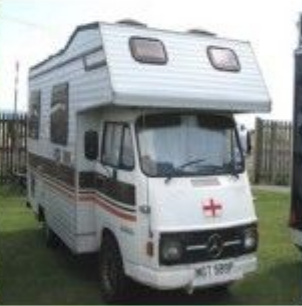
\includegraphics[scale=0.15]{images/bus.png}};
     	%	\node at (-5,3.8){\small Content Image};
     }
     
    \onslide<1->{\node[inner sep=0pt] (B) at (-1.1,4.8) {%\begin{center}
\begin{tikzpicture}[scale=0.3,transform shape]

\pgfsetxvec{\pgfpoint{1cm}{0cm}}
\pgfsetyvec{\pgfpoint{0cm}{1cm}}
\pgfsetzvec{\pgfpoint{-.5cm}{-.866cm}}

\def\cuboid#1#2#3#4#5{
\begin{scope}
\edef\mycolor{#2}
\edef\depth{#3}
\edef\height{#4}
\edef\width{#5}
\draw[black,fill=\mycolor, fill opacity=0.4, text opacity=1] #1 -- ++(-\depth,0,0) -- ++(0,-\height,0) -- ++(\depth,0,0) -- cycle #1 -- ++(0,0,-\width) -- ++(0,-\height,0) -- ++(0,0,\width) -- cycle  #1 -- ++(-\depth,0,0) -- ++(0,0,-\width) -- ++(\depth,0,0) -- cycle;
\end{scope}
}

\def\cuboidlabel#1#2#3#4#5#6#7#8{
\begin{scope}
\edef\mycolor{#2}
\edef\depth{#3}
\edef\height{#4}
\edef\width{#5}
\edef\depthlabel{#6}
\edef\heightlabel{#7}
\edef\widthlabel{#8}
\draw[draw=none,fill=\mycolor, fill opacity=0.4, text opacity=1] #1 -- ++(-\depth,0,0) -- ++(0,-\height,0) -- ++(\depth,0,0) node[black,pos=0.5,below] {\tiny \depthlabel} -- cycle #1 -- ++(0,0,-\width) -- ++(0,-\height,0) node[black,pos=0.5,right] {\tiny \heightlabel} -- ++(0,0,\width)  node[black,pos=0.5,below,right] {\tiny \widthlabel} -- cycle  #1 -- ++(-\depth,0,0) -- ++(0,0,-\width) -- ++(\depth,0,0) -- cycle;
\end{scope}
}

\def\kernel#1#2#3#4#5#6{
\begin{scope}
\edef\mycolor{#2}
\edef\depth{#3}
\edef\height{#4}
\edef\width{#5}
\draw[black,fill=\mycolor, fill opacity=0.4, text opacity=1] #1 -- ++(-\depth,0,0) -- ++(0,-\height,0) -- ++(\depth,0,0) -- cycle #1 -- ++(0,0,-\width) -- ++(0,-\height,0) -- ++(0,0,\width) -- cycle  #1 -- ++(-\depth,0,0) -- ++(0,0,-\width) -- ++(\depth,0,0) -- cycle;

\draw[dotted] #1 -- #6 #1++(0,0,-\width) -- #6 #1++(0,-\height,0) -- #6 #1++(0,-\height,-\width) -- #6;

\end{scope}
}

\def\kernellabel#1#2#3#4#5#6#7#8#9{
%#6 is target pixel
\begin{scope}
\edef\mycolor{#2}
\edef\depth{#3}
\edef\height{#4}
\edef\width{#5}
\edef\depthlabel{#7}
\edef\heightlabel{#8}
\edef\widthlabel{#9}
\draw[draw=none,fill=\mycolor, fill opacity=0.4, text opacity=1] #1 -- ++(-\depth,0,0) -- ++(0,-\height,0) -- ++(\depth,0,0) -- cycle #1 -- ++(0,0,-\width) -- ++(0,-\height,0) node[pos=0.5,left] {\tiny \heightlabel} -- ++(0,0,\width)  node[pos=0.6,above] {\tiny \widthlabel} -- cycle  #1 -- ++(-\depth,0,0) -- ++(0,0,-\width) -- ++(\depth,0,0) -- cycle;

\draw[dotted] #1 -- #6 #1++(0,0,-\width) -- #6 #1++(0,-\height,0) -- #6 #1++(0,-\height,-\width) -- #6;

\end{scope}
}

%alexnet
\cuboidlabel{(0,0,0)}{gray}{0.03}{5.5}{5.5}{3}{227}{227}
\node (a) at (-0.015,-6.2,0) {\tiny Input};

\kernellabel{(0,-1,-1)}{blue}{0.03}{1.6}{1.6}{(1.7,-2,-2)}{3}{11}{11}


\cuboidlabel{(2,-0.5,-0.5)}{red}{0.6}{4.5}{4.5}{96}{55}{55}
\node (a) at (2-0.3,-0.5-4.5-0.7,-0.5) {\tiny Convolution};

\kernellabel{(2,-1.5,-1.5)}{blue}{0.6}{0.7}{0.7}{(3.7,-2.5,-2.5)}{96}{3}{3}


\cuboidlabel{(4,-1,-1)}{yellow}{0.6}{3.5}{3.5}{96}{27}{27}
\node (a) at (4-0.3,-1-3.5-0.7,-1) {\tiny MaxPooling};

\kernellabel{(4,-2,-2)}{blue}{0.6}{1}{1}{(5.7,-3,-3)}{96}{5}{5}


\cuboidlabel{(6,-1.5,-1.5)}{red}{1}{3.3}{3.3}{256}{23}{23}
\node (a) at (6-0.5,-1.5-3.3-0.7,-1.5) {\tiny Convolution};

\kernellabel{(6,-2.5,-2.5)}{blue}{1}{0.6}{0.6}{(7.7,-3.5,-3.5)}{256}{3}{3}


\cuboidlabel{(8,-2,-2)}{yellow}{1}{2.5}{2.5}{256}{11}{11}
\node (a) at (8-0.5,-2-2.5-0.7,-2) {\tiny MaxPooling};

\kernellabel{(8,-3,-3)}{blue}{1}{0.6}{0.6}{(9.7,-3.8,-3.8)}{256}{3}{3}


\cuboidlabel{(10,-2.5,-2.5)}{red}{1.3}{2.2}{2.2}{384}{9}{9}
\node (a) at (10-0.65,-2.5-2.2-0.7,-2.5) {\tiny Convolution};

\kernellabel{(10,-3.2,-3.2)}{blue}{1.3}{0.6}{0.6}{(11.5,-3.7,-3.7)}{384}{3}{3}


\cuboidlabel{(12,-3,-3)}{red}{1.3}{1.5}{1.5}{384}{7}{7}
\node (a) at (12-0.65,-3-1.5-0.7,-3) {\tiny Convolution};

\kernellabel{(12,-3.5,-3.5)}{blue}{1.3}{0.6}{0.6}{(13,-3.9,-3.9)}{384}{3}{3}


\cuboidlabel{(13.5,-3.5,-3.5)}{red}{1}{1}{1}{256}{5}{5}
\node (a) at (13.5-0.5,-3.5-1-0.7,-3.5) {\tiny Convolution};

\kernellabel{(13.5,-3.8,-3.8)}{blue}{1}{0.6}{0.6}{(14,-5.2,-5.2)}{256}{3}{3}

%\node (a) at (13.5-0.5+1,-6.7,-3.5) {\scriptsize $S=2$,$P=0$};
%\node (a) at (13.5-0.5+1,-7.2,-3.5) {\scriptsize Parameters: 0};


\cuboidlabel{(14.5,-5,-5)}{yellow}{1}{0.5}{0.5}{256}{2}{2}
\node (a) at (14.5-0.5,-5-0.5-0.7,-5) {\tiny MaxPooling};


%\draw[dotted,->] (14.5,-5,-5) -- (18,-0.7,0);
%\node (a) at (17.5,0,0) {\tiny dense};
%\cuboid{(18.5,3,0)}{red}{0.5}{7}{0}{256}{2}{2}
%\node (a) at (18.2,-4.5,0) {\tiny 4096};


%\draw[dotted,->] (18.5,-0.7,0) -- (19+0.5,-0.7,0) node[pos=0.5,above] {\tiny dense};
%\cuboid{(19.5+0.5,3,0)}{red}{0.5}{7}{0}{256}{2}{2}
%\node (a) at (19.2+0.5,-4.5,0) {\tiny 4096};
%
%
%\draw[dotted,->] (19.5+0.5,-0.7,0) -- (20+1,-0.7,0) node[pos=0.5,above] {\tiny dense};
%\cuboid{(20.5+1,2,0)}{red}{0.5}{5}{0}{256}{2}{2}
%\node (a) at (20.2+1,-3.5,0) {\tiny 1000};
%\cuboid{(20.5+1,1,0)}{green}{0.5}{0.5}{0}{256}{2}{2}
%\node (a) at (20.2+2,0.8,0) {\small Dumbell};

\end{tikzpicture}
%\end{center}

};
     	\draw [->,thick] (-4.1,4.8) -- (-3.7,4.8);
     }
     
         \onslide<2->{
         	\node[inner sep=0pt] (A) at (2.1,4.8) {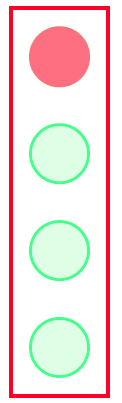
\includegraphics[scale=0.15]{images/classification.PNG}};
   	     	\draw [->,thick] (1.5,4.8) -- (2,4.8);
   	     	\node at (2.8,5.6) {\tiny ostrich};
   	     	\node at (2.8,5.2) {\vdots};
   	     	\node at (2.8,4.6) {\tiny bus};
   	     	\node at (2.8,4.3) {\vdots};
         	}
     \end{tikzpicture}
        
    \end{overlayarea}

    \column{0.5\textwidth}
    \begin{overlayarea}{\textwidth}{\textheight}
    \only<1->{
        \begin{itemize}
        	\justifying
            \item<1-> Suppose we feed in an image to a Convnet.
            \item<2-> Now instead of maximizing the log-likelihood of the correct class (bus) we set the objective to maximize some incorrect class (say, ostrich)
            \item<3-> Turns out that with minimal changes to the image (using backprop) we can soon convince the Convnet that this is an ostrich.
     	    \item<4-> Let us see some examples
        \end{itemize}
    }
    \end{overlayarea}
  \end{columns}
\end{frame}

%%%%%%%%%%%%%%%%%%%%%%%%%%%%%%%%%%%%%%%%%%%%%%%%%%%%%%%%%%%%%%%%%%%%%%%%%%%%%%%%%%%%%%%%%

\begin{frame}
  \begin{columns}
    \column{0.6\textwidth}
    \vspace{0.5cm}
        \begin{overlayarea}{\textwidth}{\textheight}
    
		\begin{tikzpicture}
		
		\onslide<1->{
		\node[inner sep=0pt] (A) at (-1,8)
		     {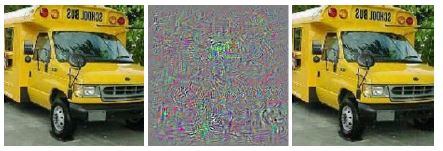
\includegraphics[scale = 0.4]{images/1}};
		     %\node at (-2,2.5) {correct};
		     %\node at (0,2.5) {+distort};
		     %\node at (2,2.5) {ostrich};
		     }
		     
		\onslide<2->{
		\node[inner sep=0pt] (A) at (-1,6)
		     {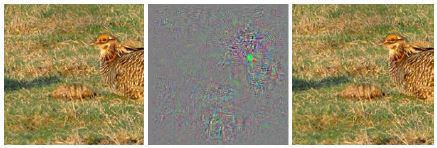
\includegraphics[scale = 0.4]{images/2}};
		     }
		     
		\onslide<3->{
		\node[inner sep=0pt] (A) at (-1,4)
		     {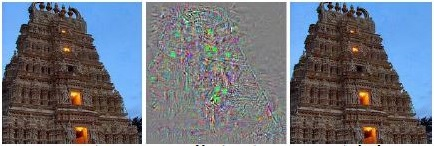
\includegraphics[scale = 0.4]{images/3}};
		     }
		     
		     \onslide<4->{
		\node[inner sep=0pt] (A) at (4,8)
		     {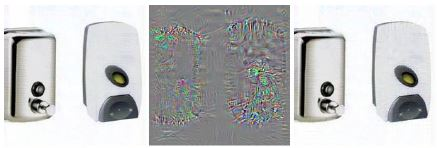
\includegraphics[scale = 0.4]{images/4}};
		     }
		     %\node at (4,2.5) {correct};
		     %\node at (6,2.5) {+distort};
		     %\node at (8,2.5) {ostrich};
		     
		   \onslide<5->{
		\node[inner sep=0pt] (A) at (4,6)
		     {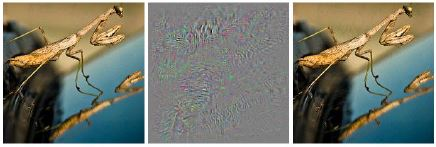
\includegraphics[scale = 0.4]{images/5}};
		     }
		     
		     \onslide<6->{
		\node[inner sep=0pt] (A) at (4,4)
		     {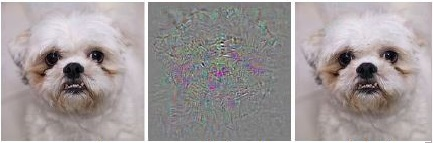
\includegraphics[scale = 0.4]{images/6}};
		     }
		\end{tikzpicture}
	\vspace{0.5cm}
    \footnotetext{$^*$Intriguing properties of neural networks, Szegedy et al., 2013}    
    \end{overlayarea}
    \column{0.35\textwidth}
    \begin{overlayarea}{\textwidth}{\textheight}
        \vspace{0.5cm}
        \hspace{0.2cm}
    \only<1->{
        \begin{itemize}
        	\justifying
            \item<1-> Notice that the changes are so minimal that the two images are indistinguishable to humans
            \item<2-> But the ConvNet thinks that the third image obtained by adding the first image to the second image is an ostrich 
        \end{itemize}
    }
    \end{overlayarea}
  \end{columns}
  \vspace{-2cm}
\end{frame}

%%%%%%%%%%%%%%%%%%%%%%%%%%%%%%%%%%%%%%%%%%%%%%%%%%%%%%%%%%%%%%%%%%%%%%%%%%%%%%%%%%%%%%%%%

\begin{frame}
  \begin{columns}
    \column{0.6\textwidth}
    \begin{overlayarea}{\textwidth}{\textheight}
    \vspace{0.5cm}
\begin{tikzpicture}

\onslide<1->{
\node[inner sep=0pt] (A) at (-1,8)
     {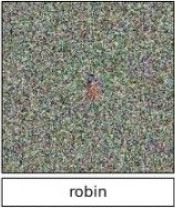
\includegraphics[scale = 0.4]{images/2_1}};
     }
     
\onslide<2->{
\node[inner sep=0pt] (A) at (1,8)
     {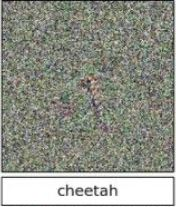
\includegraphics[scale = 0.4]{images/2_2}};
     }
     
\onslide<3->{
\node[inner sep=0pt] (A) at (3,8)
     {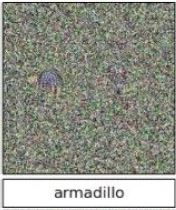
\includegraphics[scale = 0.4]{images/2_3}};
     }
     
     \onslide<4->{
\node[inner sep=0pt] (A) at (5,8)
     {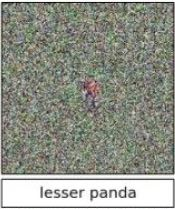
\includegraphics[scale = 0.4]{images/2_4}};
     }
     
   \onslide<5->{
\node[inner sep=0pt] (A) at (-1,5)
     {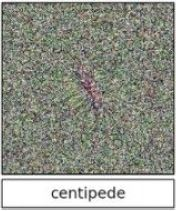
\includegraphics[scale = 0.4]{images/2_5}};
     }
     
     \onslide<6->{
\node[inner sep=0pt] (A) at (1,5)
     {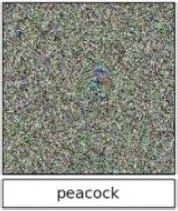
\includegraphics[scale = 0.4]{images/2_6}};
     }
     
     \onslide<7->{
\node[inner sep=0pt] (A) at (3,5)
     {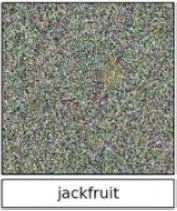
\includegraphics[scale = 0.4]{images/2_7}};
     }
     
     \onslide<8->{
\node[inner sep=0pt] (A) at (5,5)
     {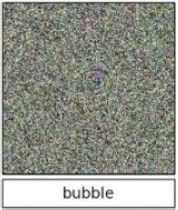
\includegraphics[scale = 0.4]{images/2_8}};
     }
     
\end{tikzpicture}
		\vspace{0.5cm}
        \footnotetext{$^*$Neural Networks are Easily Fooled: High Confidence Predictions for Unrecognizable Images
        Nguyen, Yosinski, Clune, 2014}
    \end{overlayarea}

    \column{0.4\textwidth}
        \begin{overlayarea}{\textwidth}{\textheight}
        \vspace{0.5cm}
    \only<1->{
        \begin{itemize}
        	\justifying
            \item<1-> We can also do this starting with random images and then optimizing them to predict some class.
            \item<2-> In all these cases the classifier is $99.6\%$ confident of the class
            \item<9-> Let us see an intuitive explanation of why this happens
        \end{itemize}
    }
    \end{overlayarea}
  \end{columns}
\end{frame}

%%%%%%%%%%%%%%%%%%%%%%%%%%%%%%%%%%%%%%%%%%%%%%%%%%%%%%%%%%%%%%%%%%%%%%%%%%%%%%%%%%%%%%%%%

\begin{frame}
  \begin{columns}
    \column{0.5\textwidth}
    \begin{overlayarea}{\textwidth}{\textheight}
    \vspace{0.5cm}
\begin{tikzpicture}

\onslide<1->{
\node[inner sep=0pt] (A) at (0,7)
     {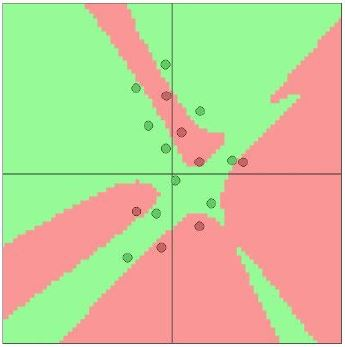
\includegraphics[scale = 0.4]{images/3_1}};
}
\onslide<6->{     
	\draw[->] (0.1,8.25) -- (2.3,10);
     \node[inner sep=0pt] (A) at (3.5,10)
     {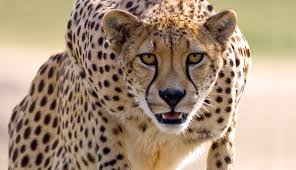
\includegraphics[scale = 0.2]{images/cheetah.jpeg}};
     
    }
\onslide<7->{    
	\draw[fill = black] (0.9,7.8) circle (0.07);
}     
\onslide<7->{     
	\draw[->] (1,7.8) -- (2.5,8);
	\node[inner sep=0pt] (A) at (3.5,8)
	{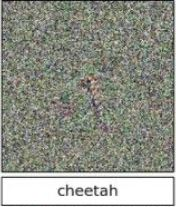
\includegraphics[scale = 0.3]{images/2_2}};
	
}

\end{tikzpicture}
        
    \end{overlayarea}

    \column{0.5\textwidth}
    \begin{overlayarea}{\textwidth}{\textheight}
    \only<1->{
        \begin{itemize}
        	\justifying
            \item<1-> Images are extremely high dimensional objects $(\mathcal{R}^{227\times227})$ 
            \item<2-> There are many many many points in this high dimensional space
     	    \item<3-> Of these only a few are images (of which we see some during training)
            \item<4-> Using these training images we fit some decision boundaries
            \item<5-> While doing so we also end up taking decisions about the  many many unseen points in this high dimensional space (Notice the large green and red regions which do not contain any training points)
        \end{itemize}
    }
    \end{overlayarea}
  \end{columns}
\end{frame}




